\documentclass{beamer}
\usepackage[english,russian]{babel}
\usepackage[utf8]{inputenc}
\usepackage{graphicx}
\usepackage{amsmath}
\usepackage{amsfonts}
\usepackage[colorlinks=true, allcolors=blue]{hyperref}
\usepackage{fancyhdr}
\usepackage{mdframed}
\usepackage{lipsum}
\usepackage{booktabs,dcolumn,caption}
\usepackage[backend=bibtex,style=authoryear]{biblatex}
%\usepackage{algorithm,algorithmic}
%\usepackage{algorithm2e}
\usepackage{algpseudocode}
\usepackage[utf8]{inputenc}
\usepackage[T1]{fontenc}
% Стиль презентации
%\usetheme{Warsaw}
\usetheme{Madrid}
\setbeamertemplate{footline}{}
\begin{document}

\title{Контрастное обучение в задачах компьютерного зрения для повышения интерпретируемости модели}
\author{Андрей Семёнов\inst{1}\inst{2}\inst{4} Владимир Иванов\inst{3} Александр Безносиков\inst{1}\inst{2}\inst{4}}
\institute{\inst{1}MIPT \quad \inst{2}Yandex Research \quad \inst{3}Innopolis University \quad \inst{4}MMO Laboratory}

\date{Май 2023} 

\begin{frame}
\maketitle
\centering
Sparse Concept Bottleneck Models: Gumbel Tricks in Contrastive Learning\\
\href{https://arxiv.org/abs/2404.03323}{https://arxiv.org/abs/2404.03323}\\
ICML 2024 submit
\end{frame}


\frame{\frametitle{Содержание}
\tableofcontents
} 
\section{Постановка задачи}

\frame{\frametitle{Concept Bottleneck модели}
%\vskip -4cm
$y \in \mathbb{R}$, $x \in \mathbb{R}^\mathrm{d}$, $c \in \mathbb{R}^{\mathrm{k}}$, $\{(x^{(i)}, y^{(i)}, c^{(i)})\}^{n}_{i=1}$, 

$g: \mathbb{R}^{\mathrm{d}} \to \mathbb{R}^{\mathrm{k}}$, $F: \mathbb{R}^{\mathrm{k}} \to \mathbb{R}$, $(F, g)$ – информационный боттлнек
\begin{itemize}
\item Independent bottleneck
$
\hat{F} = \underset{F}{\operatorname{argmin}}\sum_i\mathcal{L}_{\mathrm{Y}}(F(c^{(i)}), y^{(i)}) 
$
$
\hat{g} = \underset{g}{\operatorname{argmin}}\sum_{i, j}\mathcal{L}_{\mathrm{C_{\mathrm{j}}}}(g_\mathrm{j}(x^{(i)}))
$
\item Sequential bottleneck
$
\hat{F} = \underset{F}{\operatorname{argmin}}\sum_i\mathcal{L}_{\mathrm{Y}}(F(\hat{g}(x^{(i)})), y^{(i)})
$
\item Joint bottleneck
$
\hat{F}, \hat{g} = \underset{F, g}{\operatorname{argmin}}\sum_i\big[\lambda_1\mathcal{L}_{\mathrm{Y}}(F(g(x^{(i)}))) + \lambda_2\sum_j\mathcal{L}_{\mathrm{C_{\mathrm{j}}}}(g_{\mathrm{j}}(x^{(i)}))\big]
$
\item Standard model
$
\hat{F}, \hat{g} = \underset{F, g}{\operatorname{argmin}}\sum_i\mathcal{L}_{\mathrm{Y}}(F(g(x^{(i)})), y^{(i)})
$
\end{itemize}
}

\section{Сопутствующие работы}

\frame{\frametitle{Сопутствующие работы}
\begin{figure}[ht!]
\centering
\begin{minipage}{.5\textwidth}
  \centering
  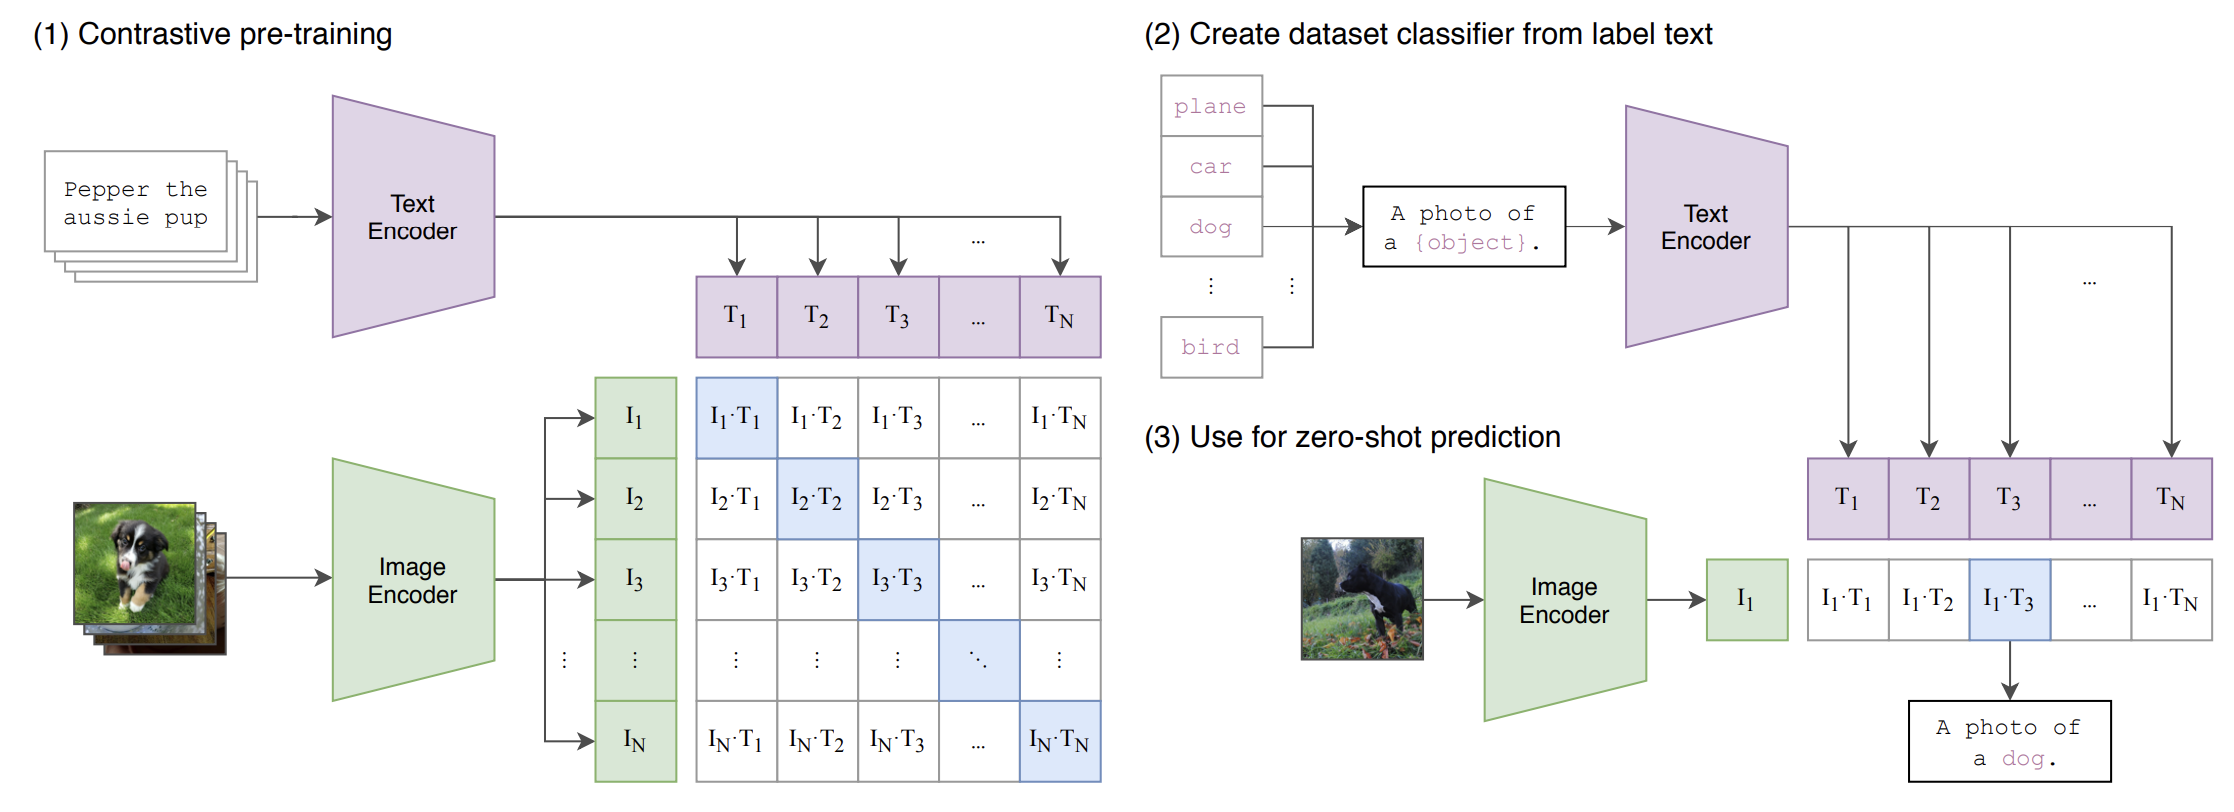
\includegraphics[width=1.\linewidth]{CLIP_arch.png}
  \captionof{figure}{CLIP}
  \label{fig:clip}
\end{minipage}%
\begin{minipage}{.5\textwidth}
  \centering
  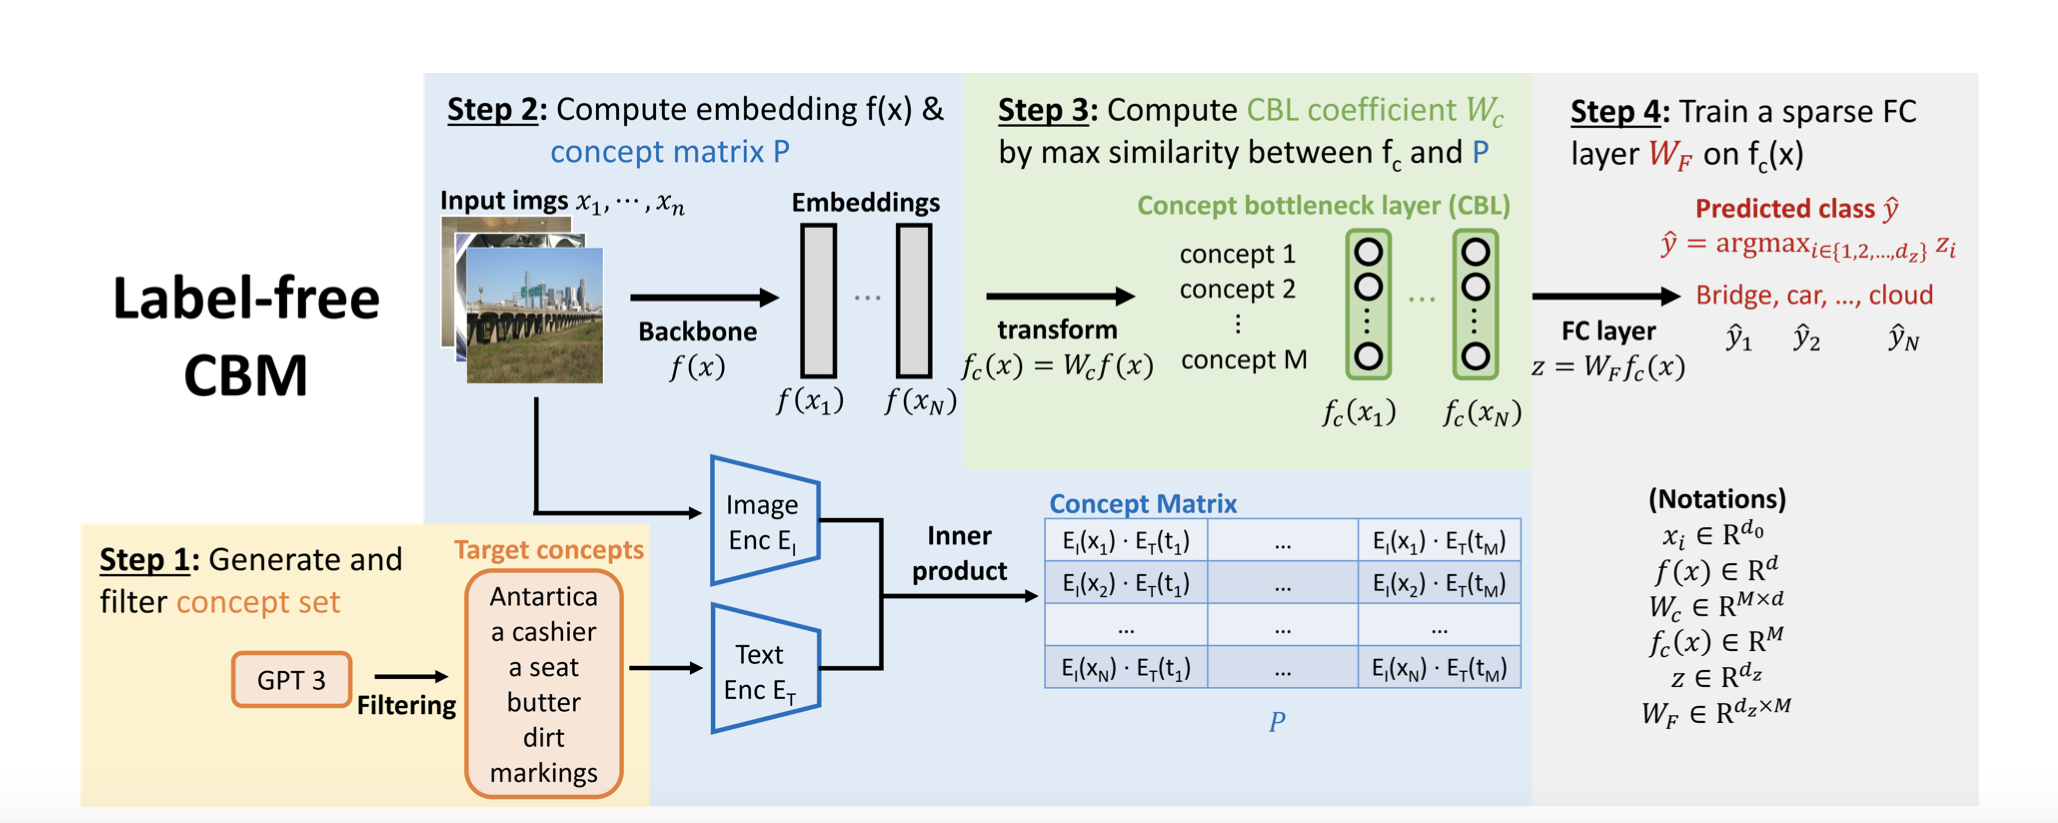
\includegraphics[width=1.\linewidth]{Label_free_CBM.png}
  \captionof{figure}{Label-free}
  \label{fig:labelfree}
\end{minipage}
\begin{minipage}{.5\textwidth}
  \centering
  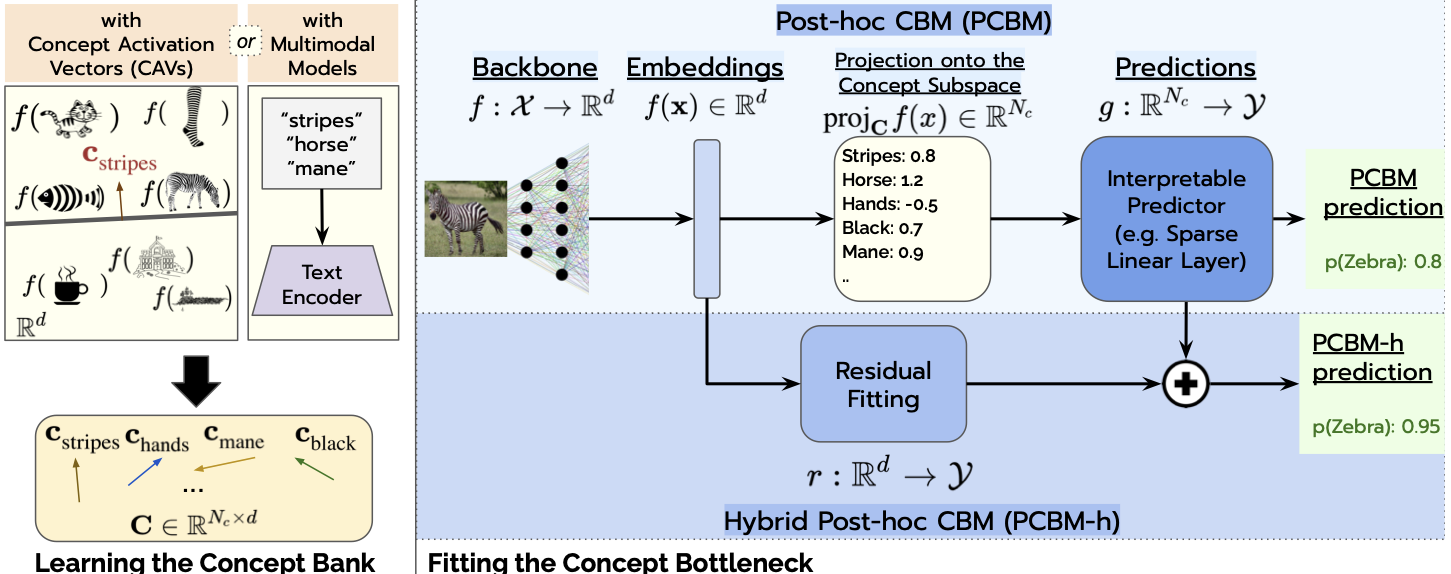
\includegraphics[width=1.\linewidth]{spring2024_pres/pcbm.png}
  \captionof{figure}{Post-hoc CBM}
  \label{fig:pcbm}
\end{minipage}
\end{figure}
}

\section{Наш вклад}

\frame{\frametitle{Наш вклад}
\begin{itemize}
\item Мы предложили два новых варианта архитектуры и алгорим для обучения Concept Bottleneck моделей (CBM).
\item Мы формально описываем алгоритм
для повышения точности CLIP – Concept Matrix Search (CMS), и в то же время
делаем модель более интерпретируемой. Мы также приводим анализ латентного пространства CLIP.
\item Получили неожиданный результат о полезности внутренних разреженных слоев в CBM.
\item Исследовали задачу распределенной оптимизации, предложили способы устранения распределений тяжелых шумов в совместной задаче NLP и CV.
\end{itemize}
}

\section{Результаты}

\subsection{Тяжелые шумы в NLP и CV}

\frame{\frametitle{Градиентный клиппинг}
\texttt{SGD}:
\begin{align}
x^{\mathrm{k+1}} = x^{\mathrm{k}} - \gamma \nabla f(x^\mathrm{k},\xi^{\mathrm{k}})
\end{align}
\texttt{Clipped-SGD}:
\begin{align}
x^{\mathrm{k+1}} = x^{\mathrm{k}} - \gamma \texttt{\textcolor{blue}{clip}}(\nabla f(x^\mathrm{k},\xi^{\mathrm{k}}), \lambda)
\end{align}
\begin{itemize}
\item $\texttt{clip}(x, 
\lambda) = \min\{1,\lambda/\|x\|\}x$
\item $\mathbb{E}_\mathrm{\xi^\mathrm{k}}[\texttt{clip}(\nabla f(x^\mathrm{k}, \lambda))]\neq\nabla f(x^\mathrm{k})$
\item При $\beta_1 = 0$ \texttt{Adam} можно интерпретировать как \texttt{Clipped-SGD} с ''адаптивным'' $\lambda$
\end{itemize}
}
\frame{\frametitle{Тяжелый шум: теоретическая справка}
Случайный вектор $X$ имеет распределение с легкими хвостами если:
\begin{align}
\mathbb{P}\{\|X-\mathbb{E}[X]\|\} \leq 2 \exp\left(-\frac{b^2}{2\sigma^2}\right) \forall b > 0,
\end{align}
что эквивалентно
\begin{align}
\mathbb{E}\Big[\exp\left(\frac{\|X-\mathbb{E}[X]\|^2}{\sigma^2}\right)\Big] \leq \exp{1}
\end{align}
Для задач с шумом в виде тяжелых хвостов в теории используют предположение:
\begin{align}
\forall \alpha\in (1,2]: \mathbb{E}[\|X-\mathbb{E}[X]\|^\mathrm{\alpha}] \leq \sigma^\mathrm{\alpha}
\end{align}
}

\frame{{Тяжелый шум: экспериментальное подтверждение}
\begin{figure}
\begin{minipage}{.45\textwidth}
  \centering
  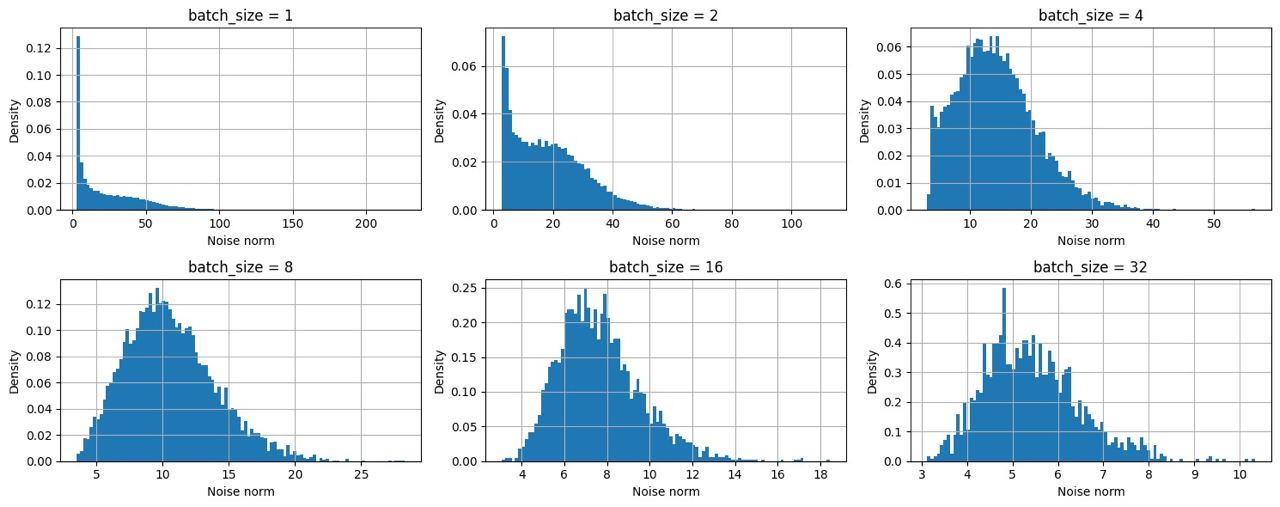
\includegraphics[width=1.\linewidth]{stoch_grads.jpg}
  \caption*{Нормы градиентов, CIFAR10.}
  \label{fig:stoch_grads}
\end{minipage}
\end{figure}

\begin{figure}[t]
        \subfloat{%
            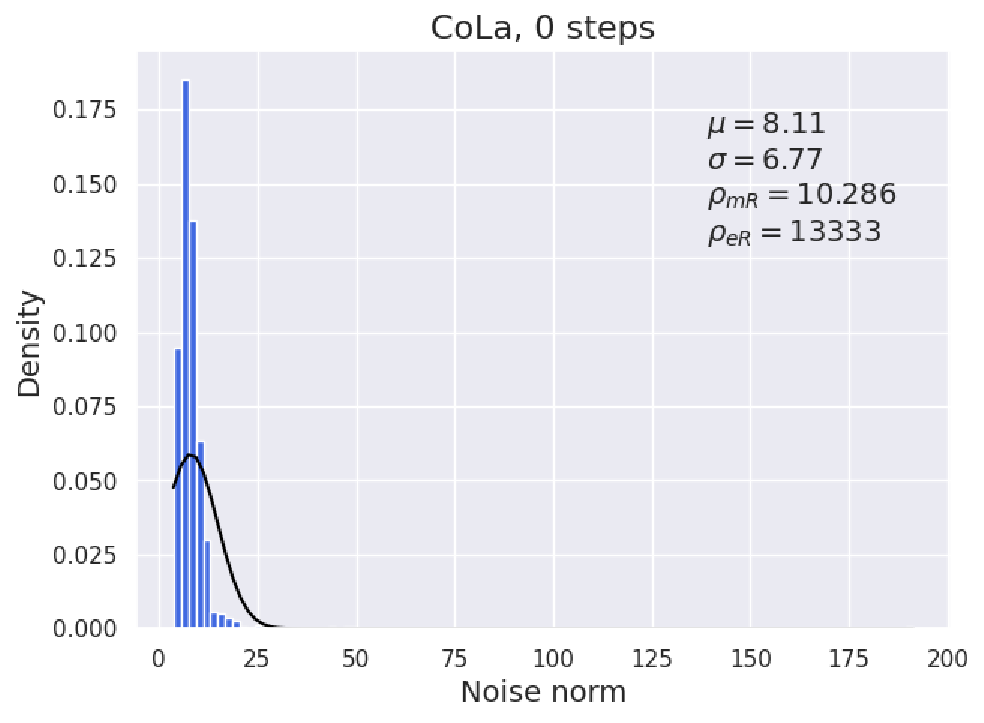
\includegraphics[width=.20\linewidth]{plots/hist_cola_0steps.pdf}%
            \label{subfig:hist_cola_0steps}%
        }
        \subfloat{%
            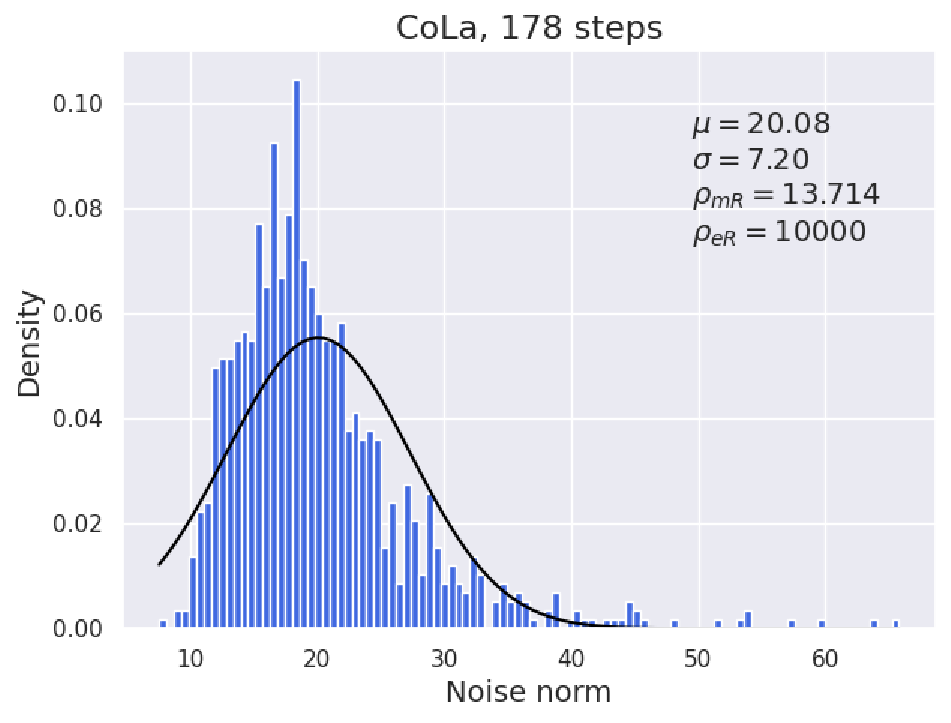
\includegraphics[width=.20\linewidth]{plots/hist_cola_178steps.pdf}%
            \label{subfig:hist_cola_178steps}%
        }
        \subfloat{%
            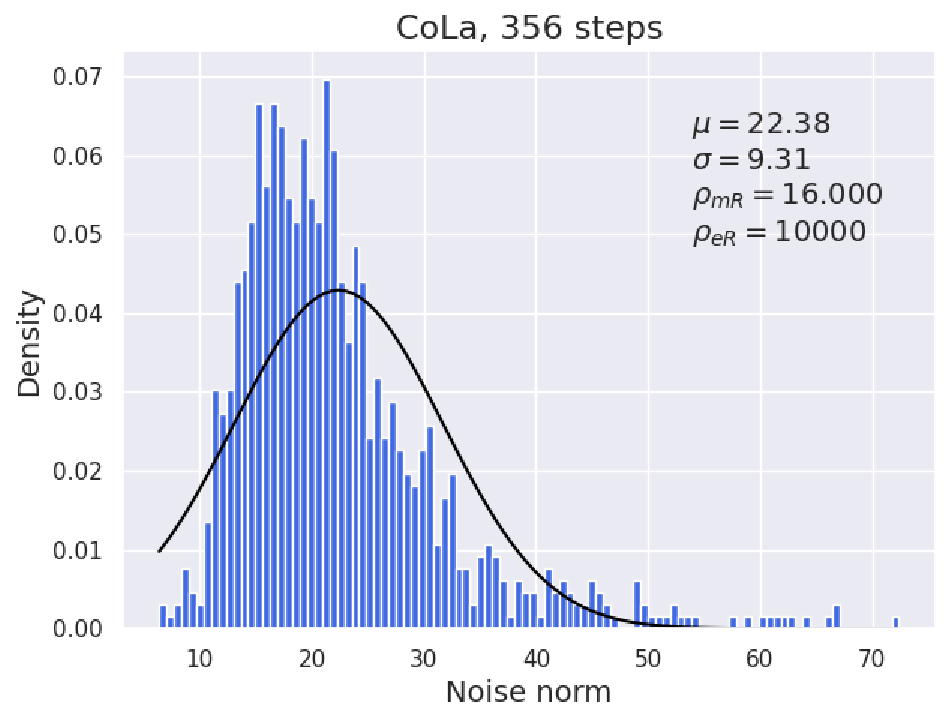
\includegraphics[width=.20\linewidth]{plots/hist_cola_356steps.pdf}%
            \label{subfig:hist_cola_356steps}%
        }
        \subfloat{%
            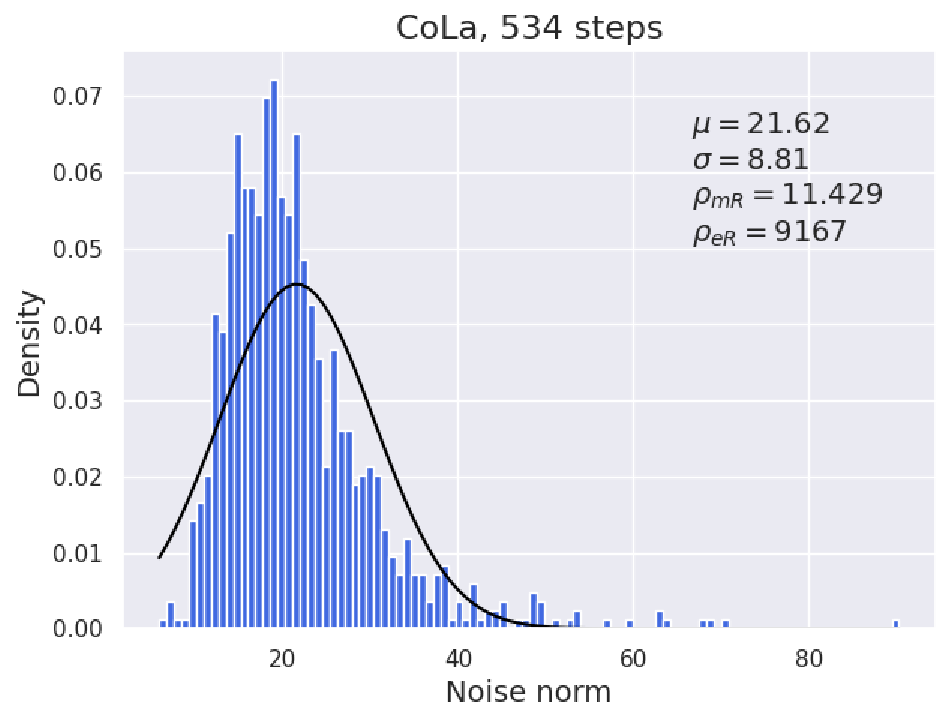
\includegraphics[width=.20\linewidth]{plots/hist_cola_534steps.pdf}%
            \label{subfig:hist_cola_534steps}%
        }\\
        \subfloat{%
            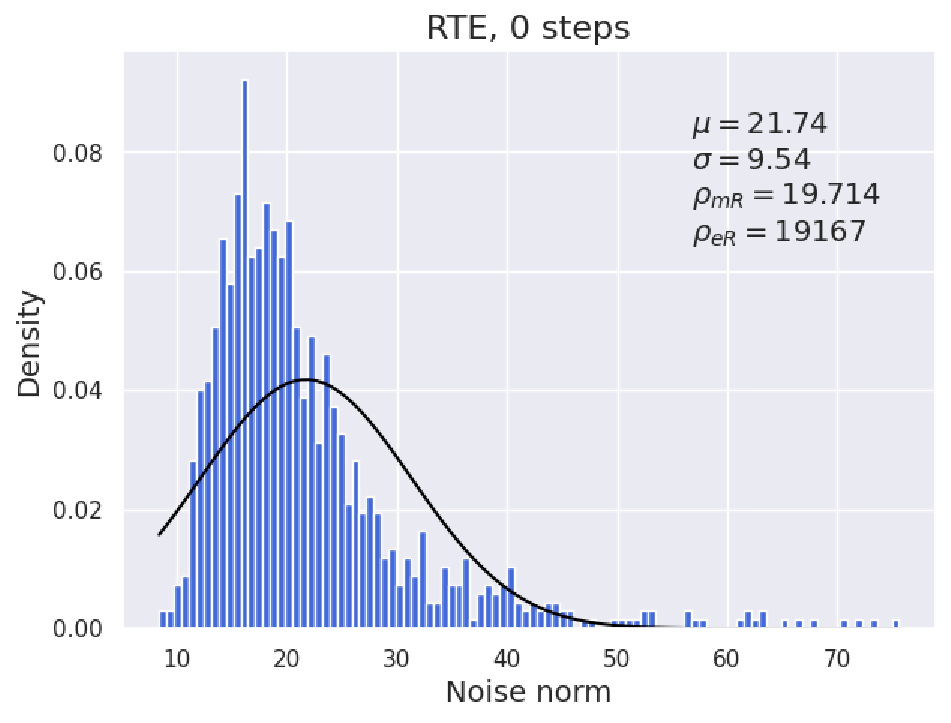
\includegraphics[width=.20\linewidth]{plots/hist_rte_0steps.pdf}%
            \label{subfig:hist_rte_0steps}%
        }
        \subfloat{%
            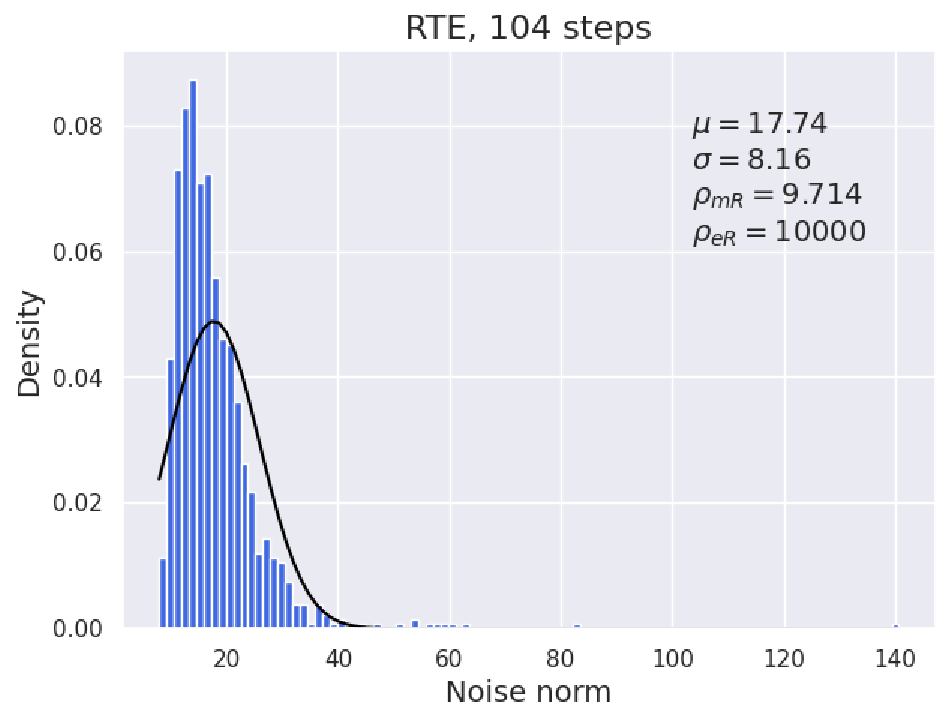
\includegraphics[width=.20\linewidth]{plots/hist_rte_104steps.pdf}%
            \label{subfig:hist_rte_104steps}%
        }
        \subfloat{%
            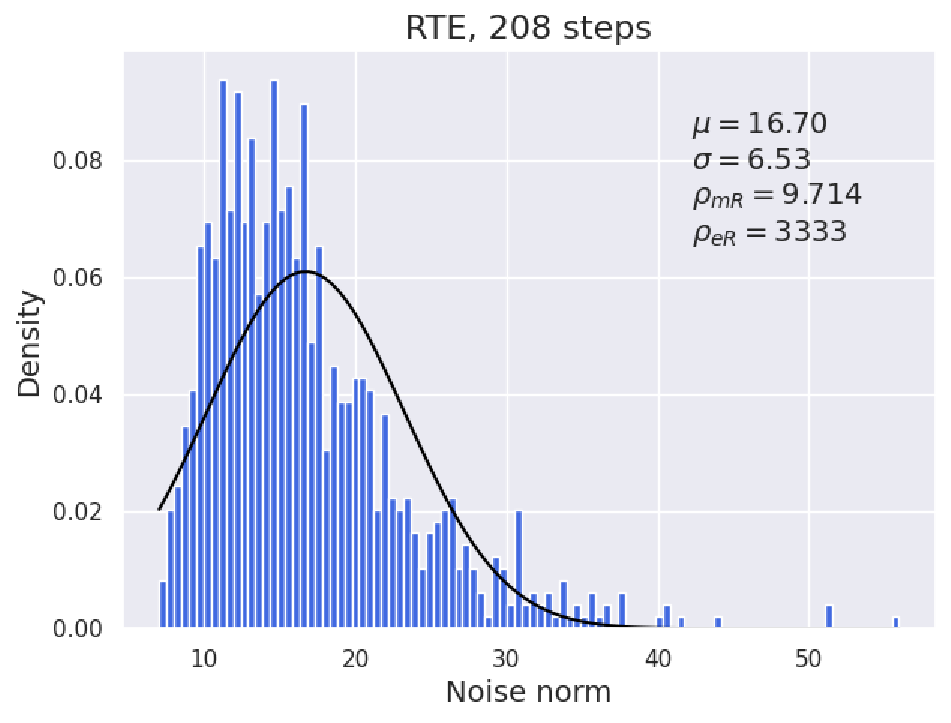
\includegraphics[width=.20\linewidth]{plots/hist_rte_208steps.pdf}%
            \label{subfig:hist_rte_208steps}%
        }
        \subfloat{%
            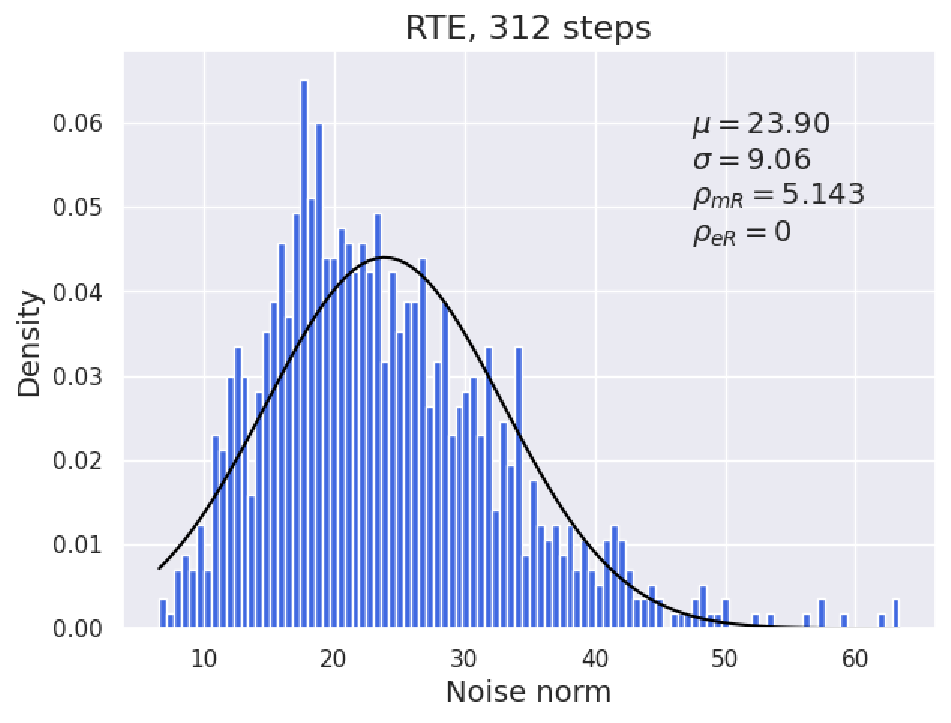
\includegraphics[width=.20\linewidth]{plots/hist_rte_312steps.pdf}%
            \label{subfig:hist_rte_312steps}%
        }\\
        \caption{Оценка градиентного шума для \texttt{Adam} на датасетах CoLa (первая строка) и RTE (вторая строка).}
        % Gradient noise evalution for \algname{Adam} on CoLa (the first row) and RTE (the second row) datasets. Histograms were evaluated after $0$ steps, after  $\approx \nicefrac{1}{3}$ and $\approx \nicefrac{2}{3}$ of all steps, and in the end.
        \label{fig:cola_rte_distribution}
\end{figure}
}

\subsection{Наш фреймворк для CBM}
\frame{\frametitle{Наша архитетура для CBM}
\begin{figure}[ht!]
\centering
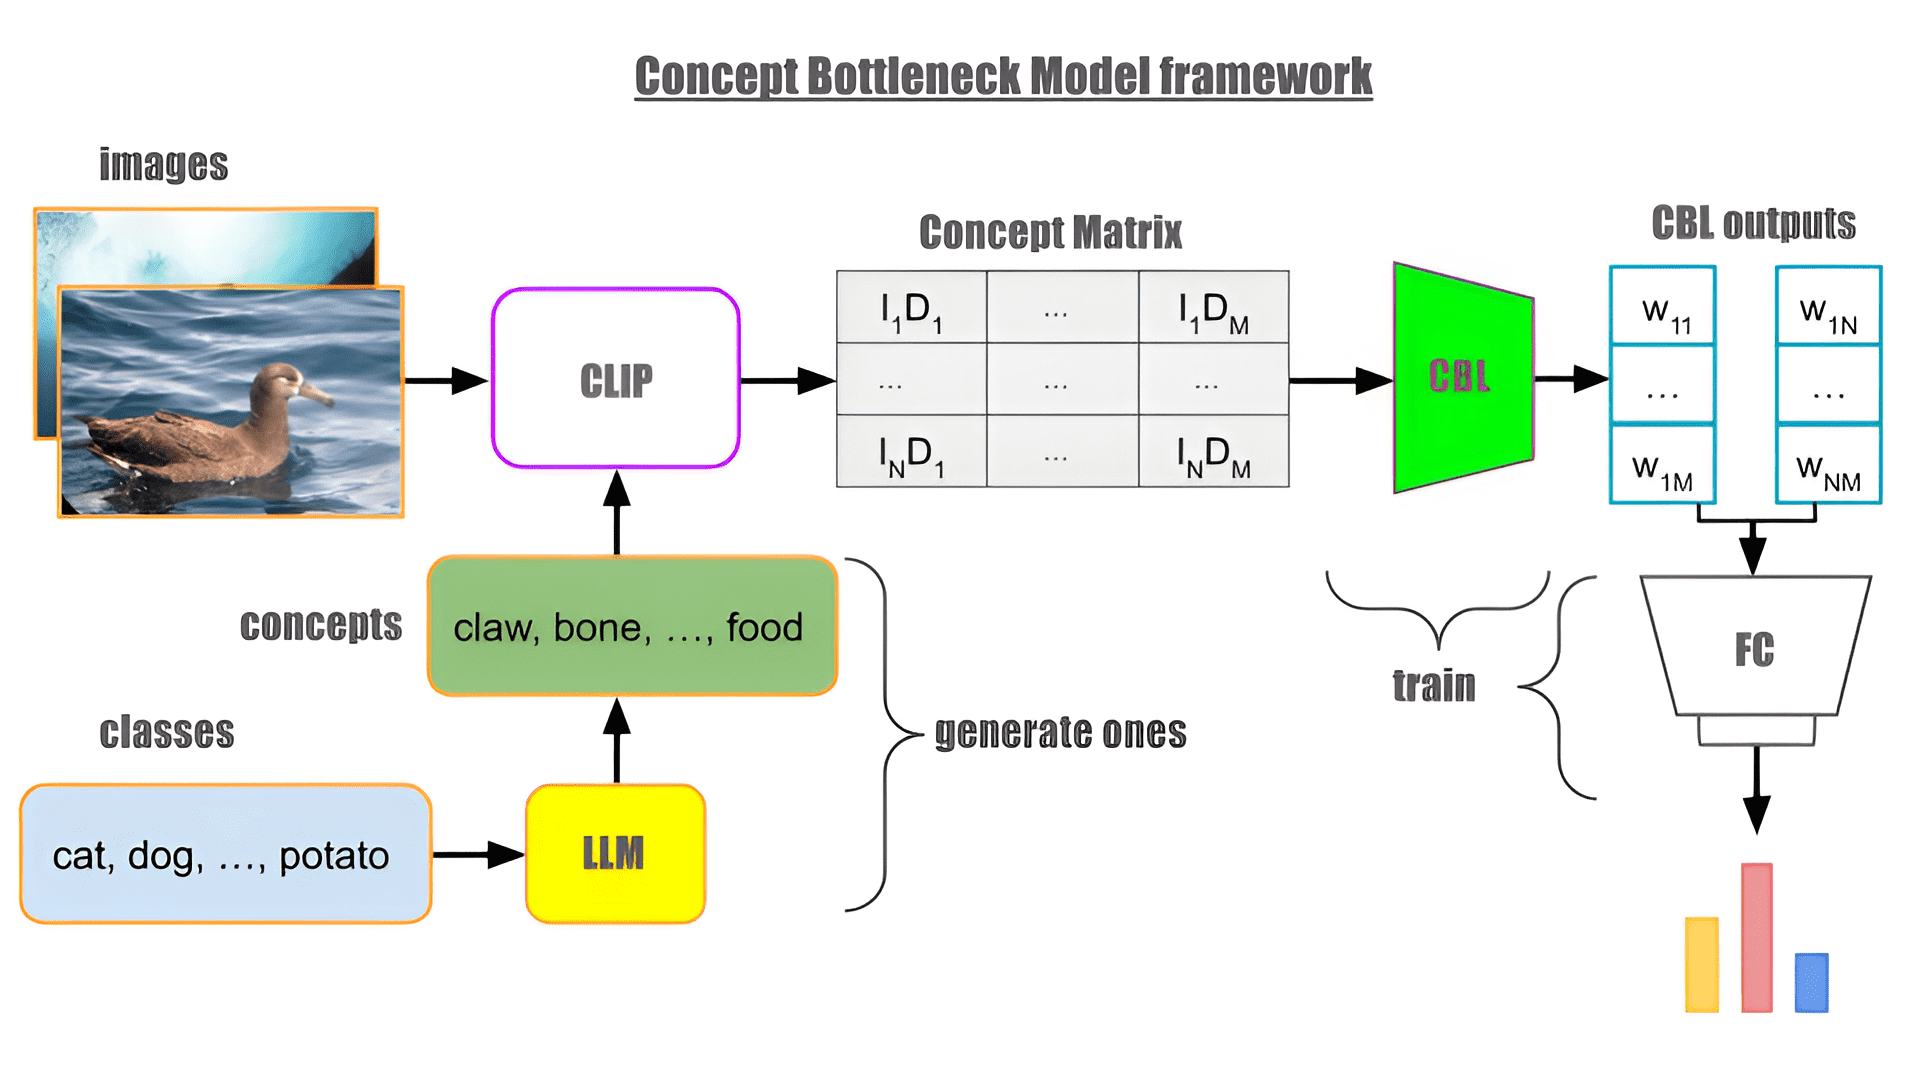
\includegraphics[width=1.\textwidth]{spring2024_pres/plots/framework-compressed.png}
\caption*{Наш CBM фреймворк.}
\label{fig:framework}
\end{figure}


% \begin{figure}[ht!]
% \centering
% \includegraphics[width=0.45\textwidth]{rule.png}
% \caption*{CMS.}
% \label{fig:arch2}
% \end{figure}
}
\subsection{Результаты Sparse-CBM, $\ell_1$-CBM, Contrastive-CBM}

\frame{\frametitle{Результаты: Общая схема для наших CBM}
\begin{itemize}
\item $i$-эмбеддинг картинки, $d$-эмбеддинг концепта, $\mathcal{D} = (x, t, l)$ – датасет.
\item CLIP: $\psi(x, t) = \left(\langle i, d_1\rangle,\dots,\langle i, d_{|\mathrm{D}|}\rangle \right)^{\mathrm{\top}} \in \mathbb{R}^{|\mathrm{D}|}$
\end{itemize}
\begin{align}
\min \limits_{W_{\mathrm{CBL}}}\mathop{\mathbb{E}}_{(x, t, l)\sim\mathcal{D}}\big[\mathcal{L}_{\mathrm{CBL}}(W_{\mathrm{CBL}}\psi(x, t))\big]_,
\end{align}
\begin{align}
\min \limits_{W_{\mathrm{F}}} \mathop{\mathbb{E}}\limits_{(x, t, l)\sim\mathcal{D}}\big[\mathcal{L}_{\mathrm{CE}}(W_{\mathrm{F}}W_{\mathrm{CBL}}\psi(x, t), l) \big]_.
\end{align}
}
\frame{\frametitle{Результаты: Contrastive-CBM}
% \begin{figure}[ht!]
% \centering
% \begin{minipage}{.5\textwidth}
%   \centering
%   \includegraphics[width=1.\linewidth]{train.jpg}
%   \caption*{Обучение с клиппингом}
%   \label{fig:train}
% \end{minipage}
% \begin{minipage}{.5\textwidth}
%   \centering
%   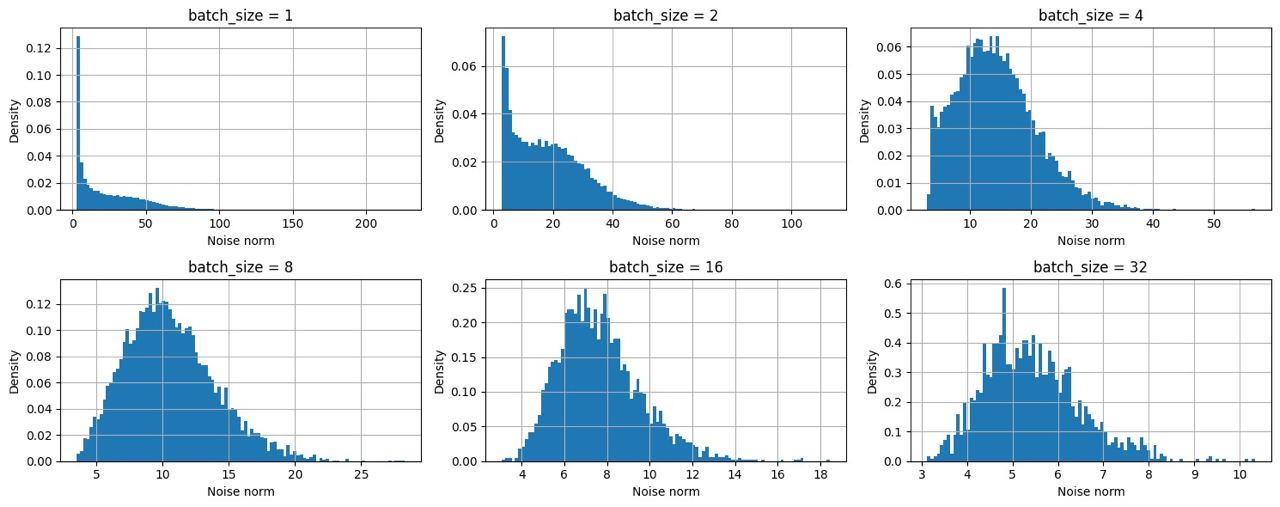
\includegraphics[width=1.\linewidth]{stoch_grads.jpg}
%   \caption*{Нормы градиентов}
%   \label{fig:stoch_grads}
% \end{minipage}
% \end{figure}}
% \subsection{Результаты CMS метода}
% \frame{\frametitle{Результаты}
% \begin{figure}[ht!]
% \centering
% \includegraphics[width=0.85\textwidth]{acc_imagenet.png}
% %\caption*{Sparse-CBM.}
% \label{fig:arch}
% \end{figure}
\textcolor{orange}{Contrastive-CBM}:
\begin{align}\label{eq:contr}
-\frac{1}{2|\mathrm{B}|} \sum_{\mathrm{k}=1}^{|\mathrm{B}|}\Bigg(\log \frac{e^{\alpha \langle w_{\mathrm{k}}, \varphi_{\mathrm{k}}\rangle}}{\sum_{\mathrm{j}=1}^{|\mathrm{B}|}e^{\alpha \langle w_{\mathrm{k}}, \varphi_{\mathrm{j}}\rangle}} + \log \frac{e^{\alpha \langle w_{\mathrm{k}}, \varphi_{\mathrm{k}}\rangle}}{\sum_{\mathrm{j}=1}^{|\mathrm{B}|}e^{\alpha \langle w_{\mathrm{j}}, \varphi_{\mathrm{k}}\rangle}} \Bigg)_.
\end{align}
}
\frame{{Результаты: Sparse-CBM}
\textcolor{orange}{Sparse-CBM}:

\begin{align}
z = \mathbf{1}\left(\arg\max \limits_{\mathrm{k}}\big[g_{\mathrm{k}} + \log \pi_{\mathrm{k}}\big] \right)_,
\end{align}

\begin{align}\label{eq:gumbellos}
-\frac{1}{2|\mathrm{B}|} \sum_{\mathrm{k}=1}^{|\mathrm{B}|}\Bigg(&\log \frac{e^{\left(\log(\alpha \langle w_{\mathrm{k}}, \varphi_{\mathrm{k}}\rangle) + g_{\mathrm{k}}\right)/\tau}}{\sum_{\mathrm{j}=1}^{|\mathrm{B}|}e^{\left(\log(\alpha \langle w_{\mathrm{k}}, \varphi_{\mathrm{j}}\rangle) + g_{\mathrm{j}}\right)/\tau}} \notag \\ 
&+ \log \frac{e^{\left(\log(\alpha \langle w_{\mathrm{k}}, \varphi_{\mathrm{k}}\rangle) + g_{\mathrm{k}}\right)/\tau}}{\sum_{\mathrm{j}=1}^{|\mathrm{B}|}e^{\left(\log(\alpha \langle w_{\mathrm{j}}, \varphi_{\mathrm{k}}\rangle) + g_{\mathrm{j}}\right)/\tau}} \Bigg)_.
\end{align}
$u \in \mathrm{Uniform}(0,1)$, $g = -\log \log u \in \mathrm{Gumbel}(0,1)$
}
\frame{{Результаты: $\ell_1$-CBM}
\textcolor{orange}{$\ell_1$-CBM}:
\begin{align}
\min \limits_{W_{\mathrm{CBL}}} \mathop{\mathbb{E}}\limits_{(x, t, l)\sim\mathcal{D}}\big[\mathcal{L}_{\mathrm{CE}}(W_{\mathrm{F}}W_{\mathrm{CBL}}\psi(x, t), l) + \frac{\lambda}{|\mathrm{D}|}\Omega(W_{\mathrm{CBL}}) \big]_,
\end{align}\label{eq:l1probl}где $\Omega(W_{\mathrm{CBL}})$ соответсвует регуляризатору. Мы используем:
\begin{align}
\Omega(W_{\mathrm{CBL}}) = \|W_{\mathrm{CBL}}\|_1
\end{align}
}

\frame{{Результаты: Concept Matrix Search алгоритм}
% \begin{algorithm}[tb]
%     \caption{\textsc{Concept Matrix Search}}
%     \label{Alg:CMS}
%     \begin{algorithmic}[1]
%     \STATE {\bfseries Input:} Batch of image embeddings $\mathrm{I_{|\mathrm{B}|}}$,  labels, all classes $\mathrm{C}$ and concepts $\mathrm{D}$ embeddings.
%     \STATE Build $\mathcal{V} \in \mathbb{R}^{|\mathrm{B}|\times |\mathrm{D}|}$, $\mathcal{T} \in \mathbb{R}^{|\mathrm{C}|\times |\mathrm{D}|}$ matrices, store $\mathcal{T}$.
%     \FOR{$\mathrm{k}=0,1,2,\dots,|\mathrm{B}|-1$}
%     \FOR{$\mathrm{m}=0,1,2,\dots,|\mathrm{C}|-1$} %\hspace{-0.3cm}
%     \STATE Compute and store $\cos(\mathcal{V}^\top_{\mathrm{k},\cdot}, \mathcal{T}^\top_{\mathrm{m},\cdot})$
%     \ENDFOR
%     \STATE Find $\mathrm{m}_{\mathrm{max}}=\underset{\mathrm{m}}{\operatorname{max}}\cos(\mathcal{V}^\top_{\mathrm{k},\cdot}, \mathcal{T}^\top_{\mathrm{m},\cdot})$
%     \IF{$\mathrm{label}(\mathrm{k}) = \mathrm{m}_{\mathrm{max}}$}
%     \STATE the hypothesis has been proven, increase Accuracy
%     \ELSE
%     \STATE the hypothesis has been disproved
%     \ENDIF
%     \ENDFOR
%     \STATE \textbf{return} Mean accuracy
% \end{algorithmic}
% \end{algorithm}
\begin{algorithm}
    \caption{\textsc{Concept Matrix Search}}
    \label{Alg:CMS}
    \begin{algorithmic}[1]
    \State {\bfseries Input:} Batch of image embeddings $\mathrm{I_{|\mathrm{B}|}}$,  labels, all classes $\mathrm{C}$ and concepts $\mathrm{D}$ embeddings.
    \State Build $\mathcal{V} \in \mathbb{R}^{|\mathrm{B}|\times |\mathrm{D}|}$, $\mathcal{T} \in \mathbb{R}^{|\mathrm{C}|\times |\mathrm{D}|}$ matrices, store $\mathcal{T}$.
    \For{$\mathrm{k}=0,1,2,\dots,|\mathrm{B}|-1$}
    \For{$\mathrm{m}=0,1,2,\dots,|\mathrm{C}|-1$}
    \State Compute and store $\cos(\mathcal{V}^\top_{\mathrm{k},\cdot}, \mathcal{T}^\top_{\mathrm{m},\cdot})$
    \EndFor
    \State Find $\mathrm{m}_{\mathrm{max}}=\underset{\mathrm{m}}{\operatorname{max}}\cos(\mathcal{V}^\top_{\mathrm{k},\cdot}, \mathcal{T}^\top_{\mathrm{m},\cdot})$
    \If{$\mathrm{label}(\mathrm{k}) = \mathrm{m}_{\mathrm{max}}$}
    \State the hypothesis has been proven, increase Accuracy
    \Else
    \State the hypothesis has been disproved
    \EndIf
    \EndFor
    \State \textbf{return} Mean accuracy
\end{algorithmic}
\end{algorithm}
}

\subsection{Сравнение с другими результатами}
\frame{\frametitle{Сравнение наших методов с предшествующими}
% \begin{table}[ht]
% \setlength\tabcolsep{0pt}
% \caption{Качество модели Sparse-CBM оносительно Label-free CBM.}
% \label{turns}
% \begin{tabular*}{\textwidth}{@{\extracolsep{\fill}} l *{3}{d{2.4}} }
% \toprule
%  %& \multicolumn{4}{c}{Datasets} \\
%  & \multicolumn{1}{c}{CIFAR10} & \multicolumn{1}{c}{CIFAR100} & \multicolumn{1}{c}{ImageNet} & \multicolumn{1}{c}{CUB} & \multicolumn{1}{c}{Places365}\\
% \midrule
% Sparse-CBM CLIP & 86.3\% & \boldsymbol{74.88\%} & 71.61\% & \boldsymbol{76.17\%} & –\\
% Label-free CBM  & \boldsymbol{86.40\%}    & 65.13\% & \boldsymbol{71.95\%} & 74.31\% & \boldsymbol{43.68\%} \\
% DescriptionCLS  &    –     &      –    &     62.97\%     &   52.57\%    &   39.90\%    \\
% \bottomrule
% \end{tabular*}
% \end{table}
\setcounter{table}{1}
\begin{table}[ht]
\caption{Сравнение перформанса Bottleneck моделей на основных датасетах. Мы наблюдаем превосходство Sparse-CBM над другими архитектурами на CIFAR10, CIFAR100 и CUB200 датасетах.}
\label{tab:cbms_tab}
\begin{center}
\vskip -0.15in
\begin{small}
\begin{sc}
\begin{tabular}{lccccr}
\toprule
Model & CIFAR10 & CIFAR100 & ImageNet & CUB200 & Places \\
\midrule
\textcolor{orange}{Sparse-CBM}    & \textbf{91.17\%} & \textbf{74.88\%} & 71.61\% & \textbf{80.02\%} & 41.34\% \\
\textcolor{orange}{$\ell_1$-CBM} & 85.11\% & 73.24\% & 71.02\% & 74.91\% & 40.87\%\\
\textcolor{orange}{Contr-CBM}  & 84.75\% & 68.46\% & 70.22\% & 67.04\% & 40.22\% \\
\texttt{[2]}    & 86.40\% & 65.13\% & \textbf{71.95\%} & 74.31\% & \textbf{43.68\%}    \\
\texttt{[3]}   &  83.34\%       &   57.20\%      &     62.57\%         &   63.92\%      &       39.66\%        \\
\texttt{[4]}             & 87.90\%&       69.10\%    &    70.40\%     & 71.80\% & 39.43\%
\\
\hline
Probing  & 96.12\%&       80.03\%     &    83.90\%     & 79.29\% & 48.33\%     \\
\bottomrule
\end{tabular}
\end{sc}
\end{small}
\end{center}
\end{table}
}
\frame{\frametitle{Сравнение Concept Matrix Search алгоритма с предшествующими методами}
\begin{table}[ht]
\caption{Сравнение CMS и "DescriptionCLS" [5]  на основных датасетах.}
\label{tab:cms_tab}
\begin{center}
\vskip -0.15in
\begin{small}
\begin{sc}
\begin{tabular}{lccccr}
\toprule
Method & CIFAR10 & CIFAR100 & ImageNet & CUB200 & Places \\
\midrule
\textcolor{orange}{CMS}    & \textbf{85.03\%} & 62.95\% & \textbf{77.82\%} & \textbf{65.17\%} & 39.43\% \\
\texttt{[5]}  &    81.61\%     &      \textbf{68.32\%}    &     75.00\%     &   63.46\%    &   40.55\%    \\
Zero-shot  &    81.79\%     &      52.84\%    &     76.20\%     &   62.63\%    &   \textbf{41.12\%}    \\
\bottomrule
\end{tabular}
\end{sc}
\end{small}
\end{center}
\vskip -0.3in
\end{table}
}
\frame{\frametitle{Визуализация пространства эмбеддингов}

\begin{figure}[h]
\begin{center}
\centerline{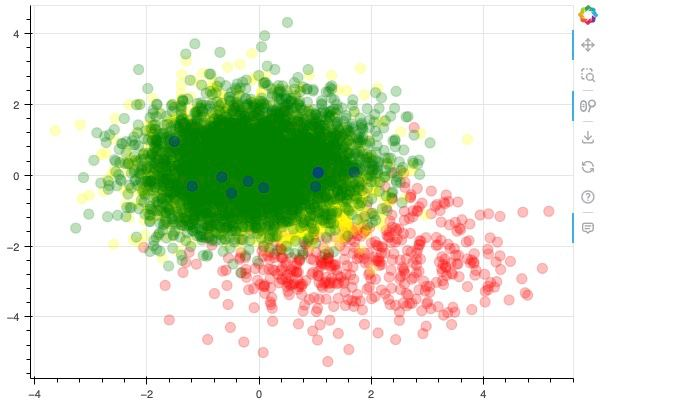
\includegraphics[width=0.5\columnwidth]{thesis/figures/cifar10tsne.jpg}} 
\caption{CIFAR10 t-SNE. Зелёные точки – проекция эмбеддингов концептов, синие  – проекция эмбеддингов классов, красные – картинки, и желтые – случайные слова.}
\label{fig:tsne}
\end{center}
\end{figure}
}
\frame{\frametitle{Визуализация CBM}
\begin{figure}[h] %ht!
\centering
   \begin{subfigure}%[b]%{3.5cm}
     \centering
    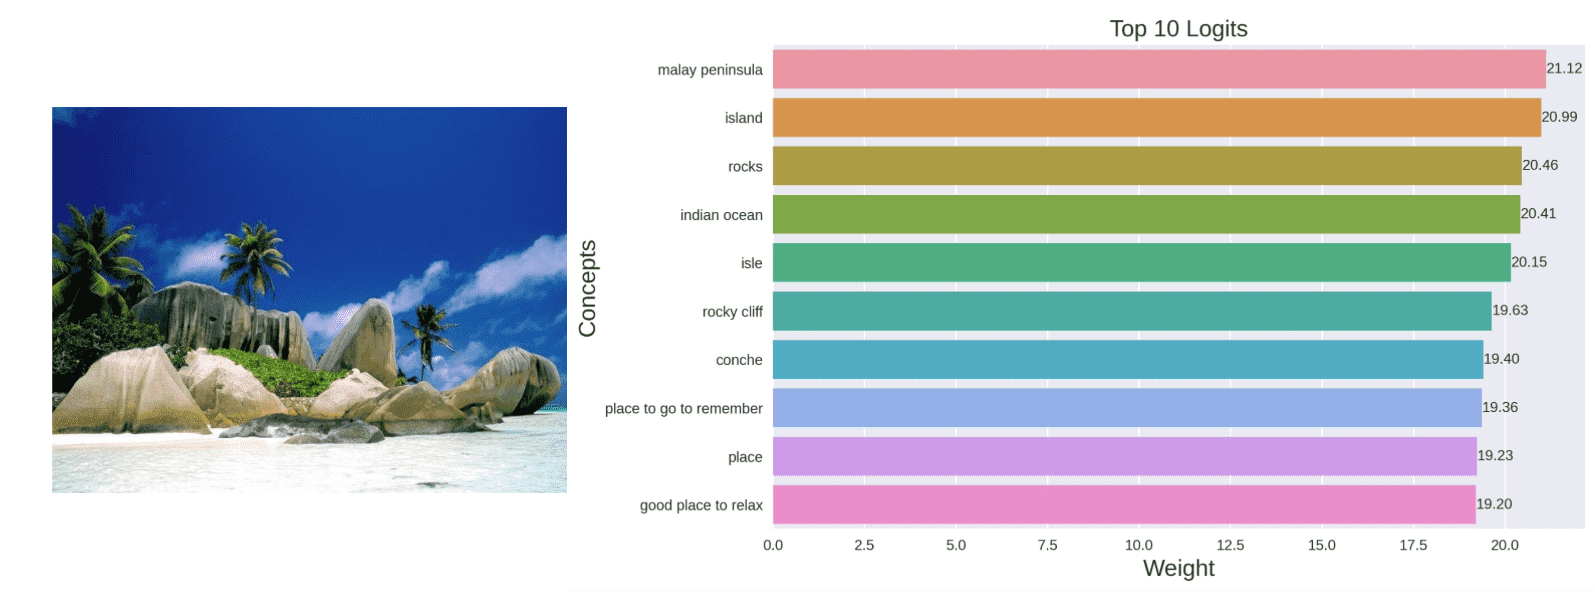
\includegraphics[width=0.75\linewidth]{thesis/figures/clip_im_1-compressed.png}
    \caption{Концепты, извлекаемые с помощью CLIP.}
    %\label{fig:clip_im_1}
    \end{subfigure}
    \begin{subfigure}%[b]%{3.5cm}
    \centering
      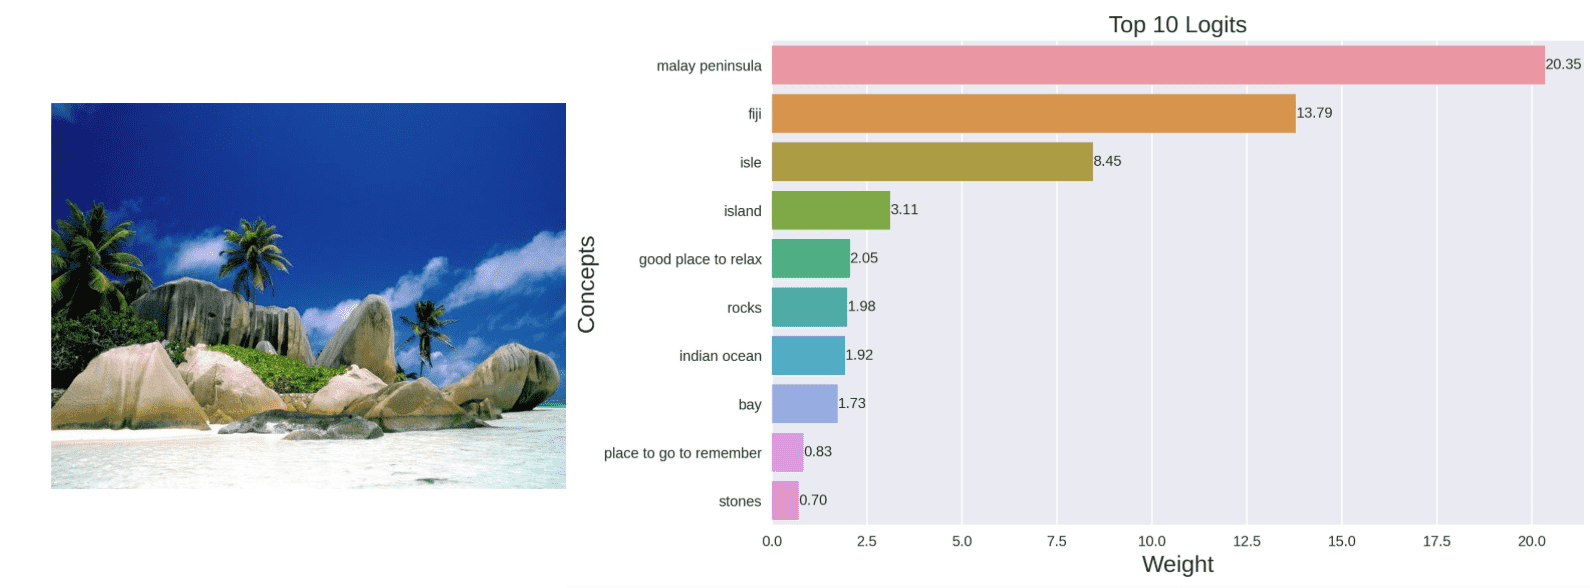
\includegraphics[width=0.75\linewidth]{thesis/figures/sparse_im_1-compressed.png}
    \caption{Концепты, извлекаемые с помощью Sparse-CBM.}
    %\label{fig:sparse_im_1}
    \end{subfigure}
\end{figure}
}
\frame{\frametitle{Визуализация CBM}
\begin{figure}[h]
    \begin{subfigure}%[b]%{3.5cm}
     \centering
  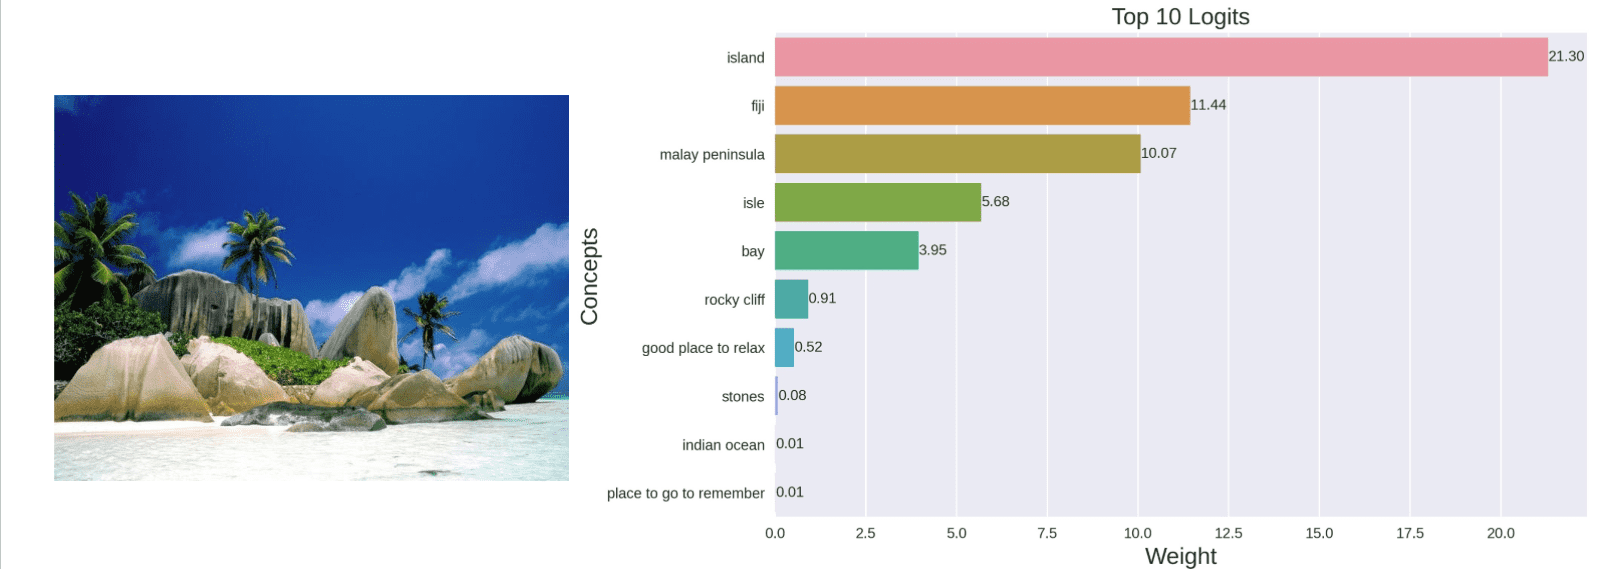
\includegraphics[width=0.75\linewidth]{thesis/figures/l1_im1-compressed.png}
    \caption{Концепты, извлекаемые с помощью $\ell_1$-CBM.}
    %\label{fig:l1_im_1}
    \end{subfigure}
        \begin{subfigure}%[b]%{3.5cm}
     \centering
  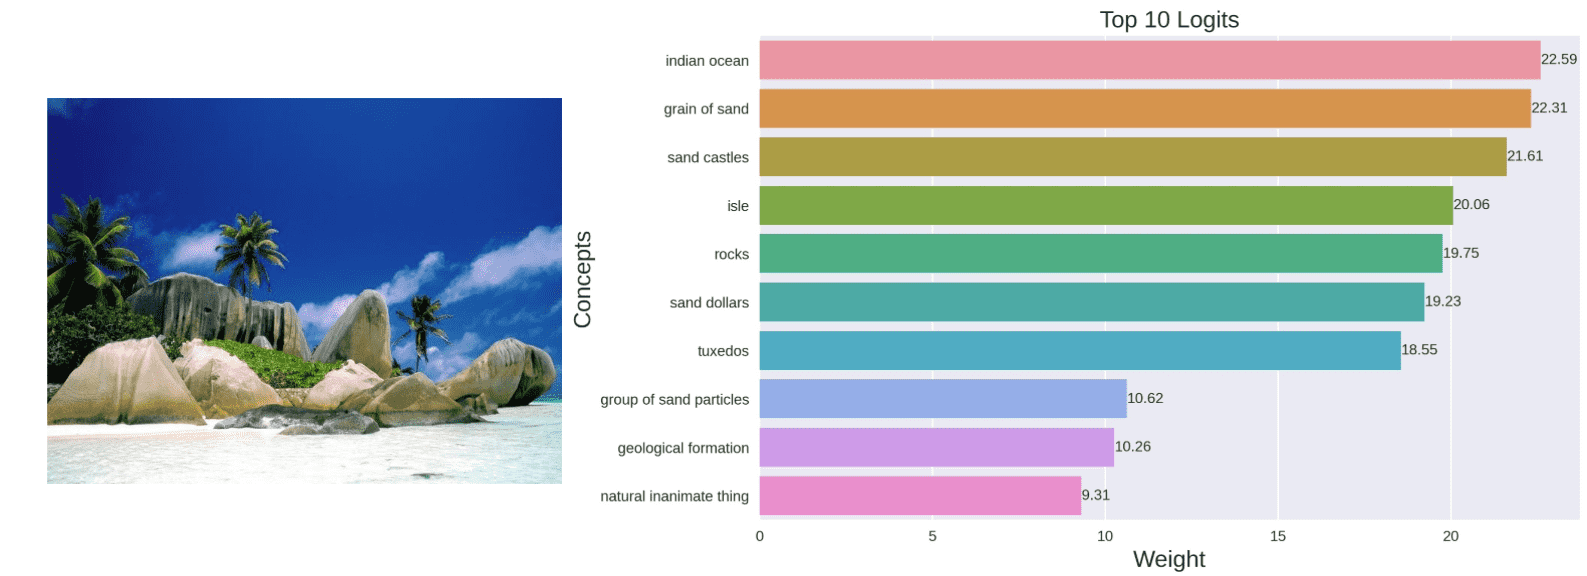
\includegraphics[width=0.75\linewidth]{thesis/figures/contr_im_1-compressed.png}
    \caption{Концепты, извлекаемые с помощью Contrastive-CBM.}
    %\label{fig:contr_im_1}
    \end{subfigure}
\end{figure}
}
\section{Ссылки на статьи из презентации}
\frame{\frametitle{Ссылки}
[1] Alec Radford, Jong Wook Kim, Chris Hallacy, Aditya Ramesh, Gabriel Goh, Sandhini Agarwal, Girish Sastry, Amanda Askell, Pamela Mishkin, Jack
Clark, Gretchen Krueger, and Ilya Sutskever. Learning transferable visual
models from natural language supervision, 2021.

[2] Tuomas Oikarinen, Subhro Das, Lam M. Nguyen, and Tsui-Wei Weng.
Label-free concept bottleneck models. In The Eleventh International Conference on Learning Representations, 2023.

[3] Yuksekgonul, M., Wang, M., and Zou, J. Post-hoc
concept bottleneck models, 2023.

[4] Yang, Y., Panagopoulou, A., Zhou, S., Jin, D., Callison-Burch, C., and Yatskar, M. Language in a bottle:
Language model guided concept bottlenecks for in-
terpretable image classification, 2023.

[5] Menon, S. and Vondrick, C. Visual classification via
description from large language models. ICLR, 2023.
}
\end{document}